\documentclass[12pt, a4paper]{article}

\usepackage{polski}
\usepackage[utf8]{inputenc}
\usepackage{amsmath}
\usepackage{amsfonts}
\usepackage{graphicx}
\usepackage[margin=0.7in]{geometry}
\usepackage{url}
\usepackage[hidelinks]{hyperref}
\usepackage{enumitem}
\usepackage{subcaption}
\usepackage{float}

\usepackage{titlesec}

\providecommand{\tightlist}{%
  \setlength{\itemsep}{0pt}\setlength{\parskip}{0pt}}

\begin{document}
\setlength{\parindent}{0pt}
\begin{titlepage}
    \centering
    \vspace{20cm}
    {\huge\bfseries TinyAd \unskip\strut\par}
    {\huge\bfseries Projekt wstępny \unskip\strut\par}
    \vspace{1cm}
    {\Large\itshape Rafał Kulus (Lider), \\Damian Kolaska, \\Kamil Przybyła \unskip\strut\par}
    \vspace{1cm}
    \href{https://bitbucket.org/BlueAlien99/tinyad}{https://bitbucket.org/BlueAlien99/tinyad}

    \vfill
    
    {\large \today\par}
\end{titlepage}
\tableofcontents
\clearpage

\hypertarget{treux15bux107-zadania}{%
\section{Treść zadania}\label{treux15bux107-zadania}}

W systemie pracuje stacja zarządzająca i zbiór (do kilkudziesięciu
tysięcy) sterowników paneli reklamowych. Stacja multicastowo dystrybuuje
treści i harmonogramy ich wyświetlania. Harmonogram określa okresy
wyświetlania i czas przechowywania. Sterowniki unicastowo raportują swój
stan i zgłaszają błędy. Błąd w transmisji multicastowej obsługiwany jest
retransmisją multi- lub unicastową w zależności od liczby otrzymanych
komunikatów NAK. System ma pracować w prywatnej sieci IPv6. Stacja
zarządzająca może wysyłać unicastowo ważne treści informacyjne do
natychmiastowego wyświetlenia przez wybrane sterowniki. Należy też
zaprojektować moduł do Wireshark umożliwiający wyświetlanie i analizę
zdefiniowanych komunikatów.

\hypertarget{format-plikuxf3w}{%
\section{Format plików}\label{format-plikuxf3w}}

\hypertarget{konfiguracja-dla-paneli}{%
\subsection{Konfiguracja dla paneli}\label{konfiguracja-dla-paneli}}

\texttt{panel\_name} i \texttt{tags} są opcjonalne i służą do
identyfikowania paneli w celu wyświetlenia ważnych treści. Są wysyłane
do stacji zarządzającej podczas rejestrowania panelu. Domyślna nazwa i
lokalizacja pliku to \texttt{./config.lfd}.
\\

\texttt{num\_retries} --- ilość ponowień komunikatu (\texttt{-1} = nie przerywaj), jeśli stacja zarządzająca nie odpowiada

\texttt{timeout} --- odstęp pomiędzy komunikatami w sekundach

\begin{verbatim}
server_ip=fe80::1234
panel_name=Lobby Front
tags=[oled][huge][orange apricot]
num_retries=5
timeout=30
\end{verbatim}

\hypertarget{harmonogram}{%
\subsection{Harmonogram}\label{harmonogram}}

\texttt{expire}, \texttt{weekday}, \texttt{hour} są opcjonalne. W
przypadku braku \texttt{expire}, zawartość nigdy nie wygaśnie. W
przypadku braku pozostałych dwóch pól, zawartość będzie wyświetlana
niezależnie od dnia tygodnia i / lub godziny. Pierwszeństwo ma pierwsza
zawartość, która spełnia wszystkie warunki. Dni tygodnia są indeksowane od 1.

\begin{verbatim}
file=./img.jpg
expire=2021.05.15 19:30
weekday=[1][2][3]
hour=[05:30-08:30][15:00-19:00]
---
file=./vids/video.mp4
expire=2021-06-30 00:00
\end{verbatim}

\hypertarget{interfejs-uux17cytkownika}{%
\section{Interfejs użytkownika}\label{interfejs-uux17cytkownika}}

\hypertarget{stacja-zarzux105dzajux105ca}{%
\subsection{Stacja zarządzająca}\label{stacja-zarzux105dzajux105ca}}

Stacja zarządzająca będzie posiadała prosty CLI. Dane mogą być wprowadzone przez użytkownika:

\begin{verbatim}
./station
$ <command1>
$ <command2>
...
$ <commandN>
\end{verbatim}

Dostępne polecenia: 

\begin{enumerate}
\def\labelenumi{\arabic{enumi}.}
\tightlist
\item \texttt{schedule\ ./my\_sched.sch} \\
Spowoduje rozesłanie nowego harmonogramu i wymaganych plików do paneli.\\ \texttt{./my\_sched.sch} to ścieżka do pliku zawierającego harmonogram.
\item \texttt{panic\ ./emergency.mkv\ -\/-name\ "Lobby\ Front"}
\item \texttt{panic\ ./emergency.mkv\ -\/-tags\ {[}oled{]}{[}huge{]}}\\
Spowoduje wysłanie ważnych treści do paneli, których nazwa to
\texttt{Lobby\ Front} lub które posiadają co najmniej jeden z podanych
tagów. Ważne treści będą wyświetlane tak długo, aż panel nie otrzyma
nowego harmonogramu poleceniem \texttt{schedule}
\item \texttt{bye} \\
Spowoduje wyłączenie stacji zarządzającej
\item \texttt{top\ 10} \\
Wyświetlenie 10 ostatnich linii logów o poziomie info lub wyższym.
\end{enumerate}

\hypertarget{panele}{%
\subsection{Panele}\label{panele}}

Panele nie będą posiadały interfejsu użytkownika. Wszystkie potrzebne
informacje będą wczytywane z prostego pliku konfiguracyjnego.

\hypertarget{pozostaux142e-zaux142oux17cenia-funkcjonalne}{%
\section{Pozostałe założenia funkcjonalne}\label{pozostaux142e-zaux142oux17cenia-funkcjonalne}}

Proces uruchomienia paneli powinien się ograniczyć tylko i wyłącznie do
startu aplikacji klienta, która sama wykona wszystkie wymagane
czynności, aby panel mógł zacząć wyświetlać zawartość.

Po udanej rejestracji panelu w stacji zarządzającej zostanie do niego
natychmiastowo wysłany ostatnio użyty harmonogram (jeśli taki istnieje), a także adres multicast do nasłuchiwania.

\hypertarget{zaux142oux17cenia-niefunkcjonalne}{%
\section{Założenia niefunkcjonalne}\label{zaux142oux17cenia-niefunkcjonalne}}

Stacje zarządzające i panele powinny sobie radzić ze wszystkimi
przewidzianymi błędami, aby zapewnić nieprzerwaną pracę, stabilność i
niezawodność, w szczególności błędy transmisji danych nie powinny
uniemożliwić poprawnego działania systemu.

\hypertarget{przypadki-uux17cycia}{%
\section{Przypadki użycia}\label{przypadki-uux17cycia}}

\hypertarget{rejestracja-panelu-reklamowego}{%
\subsection{Rejestracja panelu reklamowego}\label{rejestracja-panelu-reklamowego}}

\begin{enumerate}
\def\labelenumi{\arabic{enumi}.}
\tightlist
\item
  Użytkownik uruchamia panel reklamowy (opcjonalnie podając plik
  konfiguracyjny)
\item
  Panel rejestruje się, wysyłając komunikat stacji zarządzającej
\item
  Panel otrzymuje harmonogram i treści do wyświetlenia
\item
  Panel wyświetla zlecane treści
\end{enumerate}

\hypertarget{zarzux105dzanie-harmonogramem-oraz-wyux15bwietlanymi-treux15bciami}{%
\subsection{Zarządzanie harmonogramem oraz wyświetlanymi treściami}\label{zarzux105dzanie-harmonogramem-oraz-wyux15bwietlanymi-treux15bciami}}

\begin{enumerate}
\def\labelenumi{\arabic{enumi}.}
\tightlist
\item
  Użytkownik, za pośrednictwem stacji zarządzające, modyfikuje
  informacje o harmonogramie lub treściach
\item
  Stacja zarządzająca wysyła aktualne dane do paneli
\item
  Panele wyświetlają treści zgodnie z otrzymanym harmonogramem
\end{enumerate}

\hypertarget{zlecenie-natychmiastowego-wyux15bwietlenia-informacji}{%
\subsection{Zlecenie natychmiastowego wyświetlenia informacji}\label{zlecenie-natychmiastowego-wyux15bwietlenia-informacji}}

\begin{enumerate}
\def\labelenumi{\arabic{enumi}.}
\tightlist
\item
  Użytkownik, za pośrednictwem stacji zarządzające, zleca natychmiastowe
  wyświetlenie informacji podanej podgrupie paneli
\item
  Stacja zarządzająca wysyła treść do natychmiastowego wyświetlenia
\item
  Panele wyświetlają żądaną treść, ignorując treści wynikające z
  harmonogramu
\end{enumerate}

\hypertarget{obsux142uga-bux142ux119duxf3w}{%
\section{Obsługa błędów}\label{obsux142uga-bux142ux119duxf3w}}

\hypertarget{brak-harmonogramu-bux142ux119dny-harmonogram}{%
\subsection{Brak harmonogramu / błędny harmonogram}\label{brak-harmonogramu-bux142ux119dny-harmonogram}}

Panel będzie wyświetlał \texttt{default\ content}, w logach zostanie
zarejestrowana odpowiednia informacja i będą następowały regularne próby
uzyskania harmonogramu.

\hypertarget{stacja-zarzux105dzajux105ca-nie-odpowiada-na-komunikat}{%
\subsection{Stacja zarządzająca nie odpowiada na komunikat}\label{stacja-zarzux105dzajux105ca-nie-odpowiada-na-komunikat}}

\begin{enumerate}
\def\labelenumi{\arabic{enumi}.}
\tightlist
\item
  Cykliczne ponawianie komunikatu
\item
  Restart aplikacji po wyczerpaniu prób
\end{enumerate}

Konfigurowalne parametry zostały opisane w sekcji \ref{konfiguracja-dla-paneli}.

\hypertarget{brak-pliku-konfiguracyjnego}{%
\subsection{Brak pliku konfiguracyjnego}\label{brak-pliku-konfiguracyjnego}}

Wyświetlenie odpowiedniej informacji zwrotnej użytkownikowi i zamknięcie
aplikacji.

\hypertarget{bux142ux105d-transmisji-danych}{%
\subsection{Błąd transmisji danych}\label{bux142ux105d-transmisji-danych}}

W przypadku gdy w wyniku błędu sieciowego jeden lub więcej pakietów
zostanie zagubiony, odbiorca wyśle komunikat z prośbą o ponowne
przesłanie brakujących segmentów.

\hypertarget{ux15brodowisko-programistyczne}{%
\section{Środowisko programistyczne}\label{ux15brodowisko-programistyczne}}

Projekt zostanie zrealizowany na systemie operacyjnym Ubuntu 20.04 LTS,
w języku C++17. Do testów zostanie wykorzystana biblioteka GoogleTest, a
do debugowania programy gdb, valgrind oraz Wireshark. Do budowania
projektu zostaną wykorzystane CMake oraz g++. Do logowania użyjemy
biblioteki Loguru (\href{https://github.com/emilk/loguru}{https://github.com/emilk/loguru}).

\hypertarget{architektura}{%
\section{Architektura}\label{architektura}}

\hypertarget{stacja-zarzux105dzajux105ca-1}{%
\subsection{Stacja zarządzająca}\label{stacja-zarzux105dzajux105ca-1}}

\begin{center}
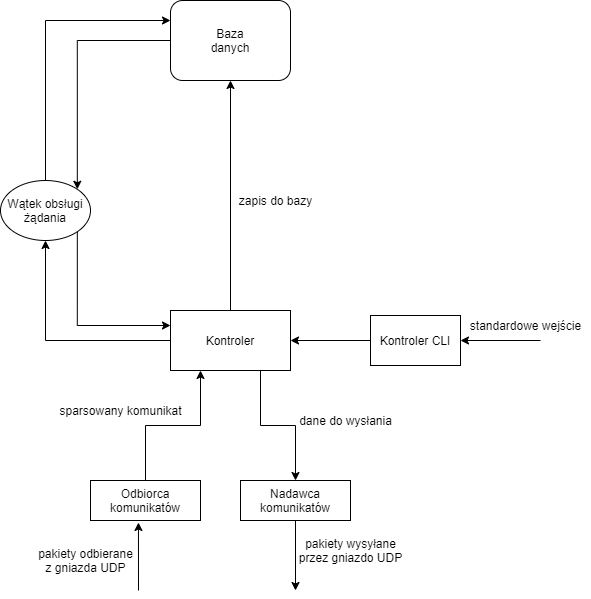
\includegraphics[width=0.55\textwidth]{9JdQG4k}
\end{center}

\hypertarget{panel}{%
\subsection{Panel}\label{panel}}

\begin{center}
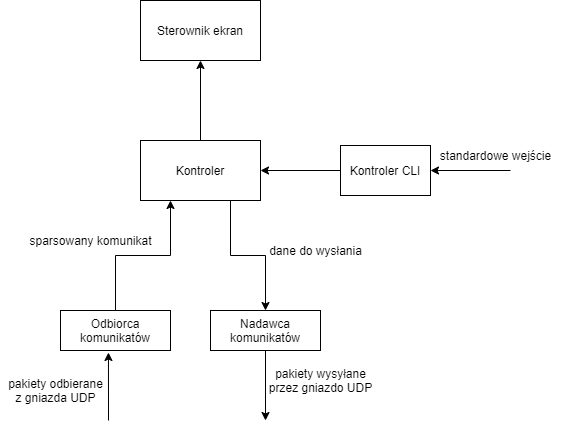
\includegraphics[width=0.55\textwidth]{W1wvgPi}
\end{center}

\textbf{Odbiorca komunikatów}: Odbiera pakiety z gniazda UDP, formuje z
nich komunikaty, weryfikuje je, a następnie wysyła do kontrolera.

\textbf{Nadawca komunikatów}: Odbiera dane od kontrolera, formuje z nich
pakiety i wysyła je przez gniazdo UDP.

\textbf{Kontroler}: Główny moduł zarządzający. Koordynuje on pracę reszty
modułów, przekierowuje komunikaty, tworzy wątki do obsługi żądań,
przekazuje polecenia do sterownika ekranu.

\textbf{Kontroler CLI}: Odbiera polecenia podawane na standardowe
wejście.

\textbf{Baza danych}: Baza danych przechowująca informacje na temat:
harmonogramu, wyświetlanych treści. Aby nie komplikować niepotrzebnie
rozwiązania użyjemy SQLite.

\hypertarget{przesyux142anie-danych}{%
\section{Przesyłanie danych}\label{przesyux142anie-danych}}

\hypertarget{architektura-komunikatuxf3w}{%
\subsection{Architektura komunikatów}\label{architektura-komunikatuxf3w}}

\hypertarget{problemy}{%
\paragraph{Problemy}\label{problemy}}

\begin{itemize}
\tightlist
\item
  jak obsłużyć komunikaty różnych typów
\item
  aby łatwo obsługiwać współbieżność, należałoby zapewnić bezstanowość
  komunikacji po stronie serwera
\item
  jak czytać komunikaty o różnych długościach
\end{itemize}

\hypertarget{rozwiux105zania}{%
\paragraph{Rozwiązania}\label{rozwiux105zania}}

\begin{itemize}
\tightlist
\item
  4 pierwsze bajty -\textgreater{} identyfikator komunikatu (np. MDAT -
  dane multimedialne)
\item
  w każdym komunikacie do serwera klient podaje czego oczekuje, np.
  trzeba dosłać fragmenty pliku o nr 3, 5, 13
\item
  czytamy po 4 bajty do momentu aż przeczytamy cały identyfikator, a
  następnie odczytamy tyle bajtów, ile zajmuje odpowiednia struktura
\end{itemize}

\hypertarget{przykux142adowy-komunikat}{%
\paragraph{Przykładowy komunikat}\label{przykux142adowy-komunikat}}

\begin{verbatim}
struct __attribute__ ((__packed__)) Multimedia {
    uint8_t tag[4] = "MDAT";
    uint8_t data[508];
};
\end{verbatim}

\hypertarget{pliki-multimedialne}{%
\subsection{Pliki multimedialne}\label{pliki-multimedialne}}

\begin{figure}[H]
\centering
  \begin{subfigure}[b]{0.48\linewidth}
    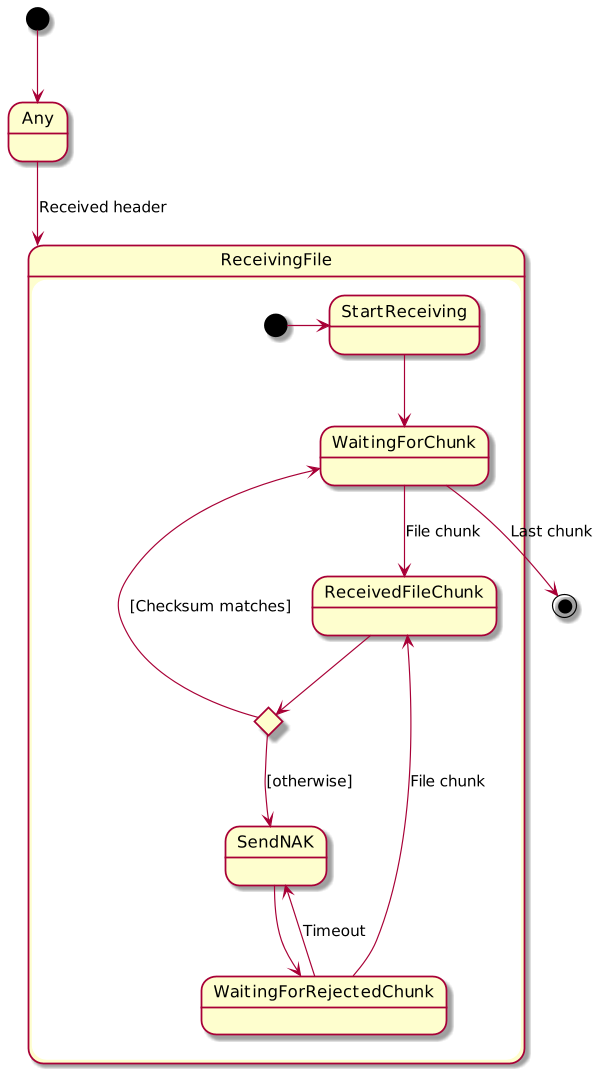
\includegraphics[width=0.7\linewidth]{client_state_diagram2.png}
    \caption{Klient}
  \end{subfigure}
  \begin{subfigure}[b]{0.48\linewidth}
    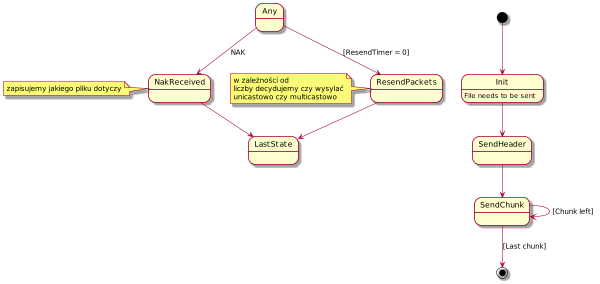
\includegraphics[width=\linewidth]{server_state_diagram2.png}
    \caption{Serwer}
  \end{subfigure}
\caption{Automaty stanów dla niezawodnej transmisji plików}
\label{fig:state_diagrams}
\end{figure}

Pliki multimedialne są zbyt duże, żeby przesyłać je w jednym datagramie.
Należy je zatem podzielić. Przesyłając plik w kawałkach, może się
okazać, że część pakietów nie dotrze albo pakiety dotrą w innej
kolejności. Aby rozwiązać ten problem zamierzamy:

\begin{itemize}
\tightlist
\item
  numerować pakiety
\item
  w każdym pakiecie podawać numer pierwszego i ostatniego pakietu w
  sekwencji
\item
  w ramach optymalizacji uprzednio podzielić pliki na kawałki i tak
  przechowywać je w bazie danych
\end{itemize}

Transmisja pliku rozpoczyna się od wysłania przez serwer wiadomości z nagłówkiem.
Nagłówek zawiera informacje takie jak: nazwa pliku, jego rozmiar, liczba części, na
które zostanie podzielony, oraz identyfikator (np. UUID), po którym będziemy rozpoznawać, czy
pakiety dotyczą danego pliku. Po wysłaniu nagłówka rozpoczyna się transmisja pliku. W ramach transmisji wysyłane
są wiadomości zawierające identyfikator (pliku), numer części, dane i sumę kontrolną. Klient odbierając pakiet danych sprawdza, czy dotyczy on obecnie przesyłanego pliku (porównując identyfikator). Następnie weryfikuje sumę kontrolną. Jeśli suma się nie zgadza, wysyła komunikat NAK do serwera.
Serwer nie odsyła pakietów od razu, a zbiera komunikaty NAK przez pewien czas, po którym decyduje, czy odesłać pakiety unicastowo czy multicastowo.

\hypertarget{sposuxf3b-testowania}{%
\section{Sposób testowania}\label{sposuxf3b-testowania}}

Do testowania wykorzystany zostanie moduł do Wiresharka, za pomocą
którego badać będziemy, czy stacja zarządzająca i panele wysyłają
odpowiednie komunikaty oraz czy ich zawartość jest zgodna z
oczekiwaniami. Na przykład podczas uruchamiania panelu, oczekiwać
będziemy, że zostanie wysłany komunikat do stacji zarządzającej, którego
zawartość będzie zgodna z konfiguracją panelu, oraz że stacja kontrolna
odeśle adekwatną odpowiedź.

Przydatne również mogą okazać się logi stacji zarządzającej, z których
będziemy mogli próbować odczytać, jakie akcje stacja wykonuje.

Przygotowane zostaną również testy regresyjne zautomatyzowane skryptami, które przetestują działanie systemu z wykorzystaniem maszyn wirtualnych symulujących stację zarządzającą i panele.

\hypertarget{sposuxf3b-demonstracji-rezultatuxf3w}{%
\section{Sposób demonstracji rezultatów}\label{sposuxf3b-demonstracji-rezultatuxf3w}}

\hypertarget{demonstracja-dziaux142ania-dystrybucji-harmonogramuxf3w-oraz-treux15bci}{%
\subsection{Demonstracja działania dystrybucji harmonogramów oraz treści}\label{demonstracja-dziaux142ania-dystrybucji-harmonogramuxf3w-oraz-treux15bci}}

\begin{enumerate}
\def\labelenumi{\arabic{enumi}.}
\tightlist
\item
  Uruchomienie stacji zarządzającej
\item
  Podłączenie panelu do działającej stacji zarządzającej
\item
  Zlecenie przesłania harmonogramu oraz treści, za pośrednictwem
  interfejsu tekstowego stacji zarządzającej
\item
  Zaprezentowanie panelu wyświetlającego wskazane treści, zgodnie z
  harmonogramem
\end{enumerate}

\hypertarget{demonstracja-dziaux142ania-dystrybucji-waux17cnych-treux15bci}{%
\subsection{Demonstracja działania dystrybucji ważnych treści}\label{demonstracja-dziaux142ania-dystrybucji-waux17cnych-treux15bci}}

\begin{enumerate}
\def\labelenumi{\arabic{enumi}.}
\tightlist
\item
  Uruchomienie stacji zarządzającej
\item
  Podłączenie kilku paneli o różnych nazwach i tagach do działającej
  stacji zarządzającej
\item
  Zlecenie wyświetlenia pilnej treści panelowi o wskazanej nazwie
\item
  Zaprezentowanie panelu wyświetlającego żądaną treść
\item
  Zlecenie wyświetlenia pilnej treści podzbiorowi paneli o wskazanym
  tagu
\item
  Zaprezentowanie paneli wyświetlających żądaną treść
\item
  Wysłanie żądania wyświetlania treści zgodnie z harmonogramem
\item
  Pokazanie paneli, wyświetlających treści według harmonogramu
\item
  Próba zlecenia wyświetlenia ważnej treści nieistniejącemu panelowi
\item
  Prezentacja informacji o nieistniejącym panelu w interfejsie tekstowym
\end{enumerate}

\hypertarget{demonstracja-dziaux142ajux105cego-mechanizmu-wyux142ux105czania-paneli}{%
\subsection{Demonstracja działającego mechanizmu wyłączania paneli}\label{demonstracja-dziaux142ajux105cego-mechanizmu-wyux142ux105czania-paneli}}

\begin{enumerate}
\def\labelenumi{\arabic{enumi}.}
\tightlist
\item
  Uruchomienie stacji zarządzającej
\item
  Podłączenie kilku paneli do działającej stacji zarządzającej
\item
  Zlecenie wyświetlenia pilnej treści panelowi o wskazanej nazwie
\item
  Zaprezentowanie paneli wyświetlających treści
\item
  Wyłączenie jednego z paneli
\item
  Zlecenie wyświetlenia pilnej treści wyłączonemu panelowi
\item
  Prezentacja informacji o nieistniejącym panelu w interfejsie tekstowym
  oraz pozostałych, działających paneli
\end{enumerate}

\hypertarget{podziaux142-prac-w-zespole}{%
\subsection{Podział prac w zespole}\label{podziaux142-prac-w-zespole}}

\begin{itemize}
\tightlist
\item
  \textbf{Rafał Kulus} -- warstwa abstrakcji na systemowe gniazda UDP
  (multicast, unicast), wielowątkowa obsługa żądań
\item
  \textbf{Damian Kolaska} -- odbieranie i nadawanie komunikatów,
  interfejs tekstowy, testy integracyjne
\item
  \textbf{Kamil Przybyła} -- moduł do Wiresharka, baza danych, obsługa harmonogramów
\end{itemize}

\hypertarget{harmonogram-prac}{%
\section{Harmonogram prac}\label{harmonogram-prac}}

\begin{itemize}
\tightlist
\item
  Do 27 kwietnia -- dokumentacja wstępna
\item
  19-26 maja -- działająca dystrybucja harmonogramów oraz wyświetlanie
  treści przez panele
\item
  Do 1 czerwca -- wysyłanie ważnych treści oraz komunikacja z warstwą
  składowania danych
\item
  Do 7 czerwca -- dokumentacja końcowa
\end{itemize}

\end{document}
